%isolated term
%#1 - Optional. Space between node and grouping line. Default=0
%#2 - node
%#3 - filling color
\newcommand{\implicantsol}[3][0]{
    \draw[rounded corners=3pt, fill=#3, opacity=0.3] ($(#2.north west)+(135:#1)$) rectangle ($(#2.south east)+(-45:#1)$);
    }


%internal group
%#1 - Optional. Space between node and grouping line. Default=0
%#2 - top left node
%#3 - bottom right node
%#4 - filling color
\newcommand{\implicant}[4][0]{
    \draw[rounded corners=3pt, fill=#4, opacity=0.3] ($(#2.north west)+(135:#1)$) rectangle ($(#3.south east)+(-45:#1)$);
    }

%group lateral borders
%#1 - Optional. Space between node and grouping line. Default=0
%#2 - top left node
%#3 - bottom right node
%#4 - filling color
\newcommand{\implicantcostats}[4][0]{
    \draw[rounded corners=3pt, fill=#4, opacity=0.3] ($(rf.east |- #2.north)+(90:#1)$)-| ($(#2.east)+(0:#1)$) |- ($(rf.east |- #3.south)+(-90:#1)$);
    \draw[rounded corners=3pt, fill=#4, opacity=0.3] ($(cf.west |- #2.north)+(90:#1)$) -| ($(#3.west)+(180:#1)$) |- ($(cf.west |- #3.south)+(-90:#1)$);
}

%group top-bottom borders
%#1 - Optional. Space between node and grouping line. Default=0
%#2 - top left node
%#3 - bottom right node
%#4 - filling color
\newcommand{\implicantdaltbaix}[4][0]{
    \draw[rounded corners=3pt, fill=#4, opacity=0.3] ($(cf.south -| #2.west)+(180:#1)$) |- ($(#2.south)+(-90:#1)$) -| ($(cf.south -| #3.east)+(0:#1)$);
    \draw[rounded corners=3pt, fill=#4, opacity=0.3] ($(rf.north -| #2.west)+(180:#1)$) |- ($(#3.north)+(90:#1)$) -| ($(rf.north -| #3.east)+(0:#1)$);
}

%group corners
%#1 - Optional. Space between node and grouping line. Default=0
%#2 - filling color
\newcommand{\implicantcantons}[2][0]{
    \draw[rounded corners=3pt, opacity=.3] ($(rf.east |- 0.south)+(-90:#1)$) -| ($(0.east |- cf.south)+(0:#1)$);
    \draw[rounded corners=3pt, opacity=.3] ($(rf.east |- 8.north)+(90:#1)$) -| ($(8.east |- rf.north)+(0:#1)$);
    \draw[rounded corners=3pt, opacity=.3] ($(cf.west |- 2.south)+(-90:#1)$) -| ($(2.west |- cf.south)+(180:#1)$);
    \draw[rounded corners=3pt, opacity=.3] ($(cf.west |- 10.north)+(90:#1)$) -| ($(10.west |- rf.north)+(180:#1)$);
    \fill[rounded corners=3pt, fill=#2, opacity=.3] ($(rf.east |- 0.south)+(-90:#1)$) -|  ($(0.east |- cf.south)+(0:#1)$) [sharp corners] ($(rf.east |- 0.south)+(-90:#1)$) |-  ($(0.east |- cf.south)+(0:#1)$) ;
    \fill[rounded corners=3pt, fill=#2, opacity=.3] ($(rf.east |- 8.north)+(90:#1)$) -| ($(8.east |- rf.north)+(0:#1)$) [sharp corners] ($(rf.east |- 8.north)+(90:#1)$) |- ($(8.east |- rf.north)+(0:#1)$) ;
    \fill[rounded corners=3pt, fill=#2, opacity=.3] ($(cf.west |- 2.south)+(-90:#1)$) -| ($(2.west |- cf.south)+(180:#1)$) [sharp corners]($(cf.west |- 2.south)+(-90:#1)$) |- ($(2.west |- cf.south)+(180:#1)$) ;
    \fill[rounded corners=3pt, fill=#2, opacity=.3] ($(cf.west |- 10.north)+(90:#1)$) -| ($(10.west |- rf.north)+(180:#1)$) [sharp corners] ($(cf.west |- 10.north)+(90:#1)$) |- ($(10.west |- rf.north)+(180:#1)$) ;
}

%Empty Karnaugh map 4x4
\newenvironment{Karnaugh}%
{
\begin{tikzpicture}[baseline=(current bounding box.north),scale=0.8]
\draw (0,0) grid (4,4);
\draw (0,4) -- node [pos=0.7,above right,anchor=south west] {AB} node [pos=0.7,below left,anchor=north east] {CD} ++(135:1);
%
\matrix (mapa) [matrix of nodes,
        column sep={0.8cm,between origins},
        row sep={0.8cm,between origins},
        every node/.style={minimum size=0.3mm},
        anchor=8.center,
        ampersand replacement=\&] at (0.5,0.5)
{
                       \& |(c00)| 00         \& |(c01)| 01         \& |(c11)| 11         \& |(c10)| 10         \& |(cf)| \phantom{00} \\
|(r00)| 00             \& |(0)|  \phantom{0} \& |(1)|  \phantom{0} \& |(3)|  \phantom{0} \& |(2)|  \phantom{0} \&                     \\
|(r01)| 01             \& |(4)|  \phantom{0} \& |(5)|  \phantom{0} \& |(7)|  \phantom{0} \& |(6)|  \phantom{0} \&                     \\
|(r11)| 11             \& |(12)| \phantom{0} \& |(13)| \phantom{0} \& |(15)| \phantom{0} \& |(14)| \phantom{0} \&                     \\
|(r10)| 10             \& |(8)|  \phantom{0} \& |(9)|  \phantom{0} \& |(11)| \phantom{0} \& |(10)| \phantom{0} \&                     \\
|(rf) | \phantom{00}   \&                    \&                    \&                    \&                    \&                     \\
};
}%
{
\end{tikzpicture}
}

%Empty Karnaugh map 2x4
\newenvironment{Karnaughvuit}%
{
\begin{tikzpicture}[baseline=(current bounding box.north),scale=0.8]
\draw (0,0) grid (4,2);
\draw (0,2) -- node [pos=0.7,above right,anchor=south west] {bc} node [pos=0.7,below left,anchor=north east] {a} ++(135:1);
%
\matrix (mapa) [matrix of nodes,
        column sep={0.8cm,between origins},
        row sep={0.8cm,between origins},
        every node/.style={minimum size=0.3mm},
        anchor=4.center,
        ampersand replacement=\&] at (0.5,0.5)
{
                      \& |(c00)| 00         \& |(c01)| 01         \& |(c11)| 11         \& |(c10)| 10         \& |(cf)| \phantom{00} \\
|(r00)| 0             \& |(0)|  \phantom{0} \& |(1)|  \phantom{0} \& |(3)|  \phantom{0} \& |(2)|  \phantom{0} \&                     \\
|(r01)| 1             \& |(4)|  \phantom{0} \& |(5)|  \phantom{0} \& |(7)|  \phantom{0} \& |(6)|  \phantom{0} \&                     \\
|(rf) | \phantom{00}  \&                    \&                    \&                    \&                    \&                     \\
};
}%
{
\end{tikzpicture}
}

%Empty Karnaugh map 2x2
\newenvironment{Karnaughquatre}%
{
\begin{tikzpicture}[baseline=(current bounding box.north),scale=0.8]
\draw (0,0) grid (2,2);
\draw (0,2) -- node [pos=0.7,above right,anchor=south west] {b} node [pos=0.7,below left,anchor=north east] {a} ++(135:1);
%
\matrix (mapa) [matrix of nodes,
        column sep={0.8cm,between origins},
        row sep={0.8cm,between origins},
        every node/.style={minimum size=0.3mm},
        anchor=2.center,
        ampersand replacement=\&] at (0.5,0.5)
{
          \& |(c00)| 0          \& |(c01)| 1  \\
|(r00)| 0 \& |(0)|  \phantom{0} \& |(1)|  \phantom{0} \\
|(r01)| 1 \& |(2)|  \phantom{0} \& |(3)|  \phantom{0} \\
};
}%
{
\end{tikzpicture}
}

%Defines 8 or 16 values (0,1,X)
\newcommand{\contingut}[1]{%
\foreach \x [count=\xi from 0]  in {#1}
     \path (\xi) node {\x};
}

%Places 1 in listed positions
\newcommand{\minterms}[1]{%
    \foreach \x in {#1}
        \path (\x) node {1};
}

%Places 0 in listed positions
\newcommand{\maxterms}[1]{%
    \foreach \x in {#1}
        \path (\x) node {0};
}

%Places X in listed positions
\newcommand{\indeterminats}[1]{%
    \foreach \x in {#1}
        \path (\x) node {X};
}



\section{Ejercicio 4: Conversor de binario a Gray de 4 bits}

\subsection{Tabla de verdad}
En la siguiente tabla se muestra la equivalencia entre un n\'umero binario de 4 bits y el mismo en c\'odigo de Gray. Seg\'un la convenci\'on adpotada, "A" ser\'a el MSB y "D" ser\'a el LSB.

\begin{table}[h!]\caption{Tabla de verdad}
\centering
\begin{tabular}{cccc|cccc}
A & B & C & D & $s_{1}$ & $s_{2}$ & $s_{3}$ & $s_{4}$ \\ \hline
0 & 0 & 0 & 0 & 0  & 0  & 0  & 0  \\
0 & 0 & 0 & 1 & 0  & 0  & 0  & 1  \\
0 & 0 & 1 & 0 & 0  & 0  & 1  & 1  \\
0 & 0 & 1 & 1 & 0  & 0  & 1  & 0  \\
0 & 1 & 0 & 0 & 0  & 1  & 1  & 0  \\
0 & 1 & 0 & 1 & 0  & 1  & 1  & 1  \\
0 & 1 & 1 & 0 & 0  & 1  & 0  & 1  \\
0 & 1 & 1 & 1 & 0  & 1  & 0  & 0  \\
1 & 0 & 0 & 0 & 1  & 1  & 0  & 0  \\
1 & 0 & 0 & 1 & 1  & 1  & 0  & 1  \\
1 & 0 & 1 & 0 & 1  & 1  & 1  & 1  \\
1 & 0 & 1 & 1 & 1  & 1  & 1  & 0  \\
1 & 1 & 0 & 0 & 1  & 0  & 1  & 0  \\
1 & 1 & 0 & 1 & 1  & 0  & 1  & 1  \\
1 & 1 & 1 & 0 & 1  & 0  & 0  & 1  \\
1 & 1 & 1 & 1 & 1  & 0  & 0  & 0 
\end{tabular}
\end{table}

En base a esto, se puede expresar a cada bit de salida ($s_{1}$,$s_{2}$,$s_{3}$,$s_{4}$) como una combinación de entradas (A,B,C,D) en forma de minitérminos.

De esta forma, obtenemos las siguientes expresiones:

\begin{equation}\label{s1_mini}
    s_{1} = A.\overline{B}.\overline{C}.\overline{D} +A.\overline{B}.\overline{C}.D+A.\overline{B}.C.\overline{D}+A.\overline{B}.C.D+A.B.\overline{C}.\overline{D}+A.B.\overline{C}.D+A.B.C.D
\end{equation}

\begin{equation}\label{s2_mini}
    s_{2} = A\overline{B}\overline{C}\overline{D} +A\overline{B}\overline{C}D+A\overline{B}C\overline{D}+A\overline{B}CD+AB\overline{C}\overline{D}+AB\overline{C}D+ABCD
\end{equation}

\begin{equation}\label{s3_mini}
    s_{3} = \overline{A}\overline{B}C\overline{D}+\overline{A}\overline{B}CD+\overline{A}B\overline{C}\overline{D}+\overline{A}B\overline{C}D+A\overline{B}C\overline{D}+A\overline{B}CD+AB\overline{C}\overline{D}+AB\overline{C}D
\end{equation}

\begin{equation}\label{s4_mini}
    s_{4} = \overline{A}\overline{B}\overline{C}D+\overline{A}\overline{B}C\overline{D}+\overline{A}B\overline{C}D+\overline{A}BC\overline{D}++A\overline{B}\overline{C}D+A\overline{B}C\overline{D}+AB\overline{C}D+ABC\overline{D}
\end{equation}

\subsection{Simplificaci\'on. Mapas de Karnaugh}

Las expresiones calculadas en el apartado anterior no son del todo eficientes a la hora de implementar el circuito l\'ogico, debido a que no están apropiadamente simplificadas. Para encontrar la expresión óptima que satisfaga la tabla de verdad utilizaremos el método de mapas de Karnaugh, en este caso con minitérminos. Como tenemos cuatro salidas distintas debemos realizar cuatro de estos mapas, que resultarán en una expresi\'on de suma de productos de las entradas. A continuaci\'on se reproducen estos diagramas y las expresiones derivadas de los mismos, donde en cada mapa cada color representa un grupo.

\begin{center}

    \begin{Karnaugh}\label{Karnaugh_s1}
        \contingut{0,0,1,1,0,0,1,1,0,0,1,1,0,0,1,1}
       \implicant{3}{10}{red}
    \end{Karnaugh}
    
Mapa de Karnaugh para S1

\begin{Karnaugh}\label{Karnaugh_s2}
        \contingut{0,1,1,0,0,1,1,0,0,1,1,0,0,1,1,0}
       \implicant{1}{9}{green}
       \implicant{2}{10}{red}
    \end{Karnaugh}
    
Mapa de Karnaugh para S2

\begin{Karnaugh}\label{Karnaugh_s4}
        \contingut{0,1,0,1,0,1,0,1,1,0,1,0,1,0,1,0}
       \implicant{1}{7}{red}
       \implicantcostats{12}{10}{green}
     \end{Karnaugh}
    
Mapa de Karnaugh para S3

\begin{Karnaugh}\label{Karnaugh_s4}
        \contingut{0,0,0,0,1,1,1,1,1,1,1,1,0,0,0,0}
       \implicant{4}{6}{red}
       \implicant{8}{10}{green}
    \end{Karnaugh}

Mapa de Karnaugh para S4    
\end{center} 
Realizando las correspondientes asociaciones obtenemos las siguientes expresiones que describen el comportamiento de cada bit de salida.

\begin{equation}\label{s1_Karnaugh}
    s_{1}= A
\end{equation}

\begin{equation}\label{s2_Karnaugh}
    s_{2}= A.\overline{B}+\overline{A}.B
\end{equation}

\begin{equation}\label{s3_Karnaugh}
    s_{3}= B.\overline{C}+\overline{B}.C
\end{equation}

\begin{equation}\label{s4_Karnaugh}
    s_{4}= C.\overline{D}+\overline{C}.D
\end{equation}

\subsection{Circuito l\'ogico}\label{ej2_circ}

En base a las ecuaciones encontradas se construy\'o el circuito l\'ogico mostrado en la figura~\ref{fig:ej4_circuito_logico}, utilizando compuertas \textsc{OR}, \textsc{AND} y \textsc{NOT}.

\begin{figure}[H]
    \centering
    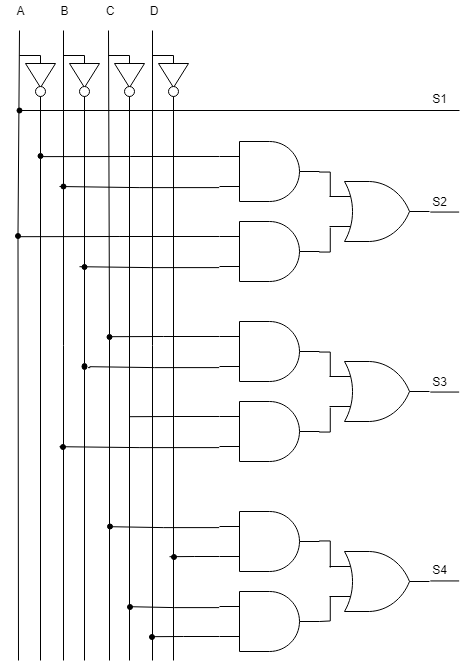
\includegraphics[width=0.9\textwidth]{./EJ_4/EJ4_TP1_Electro3.png}
    \caption{Circuito l\'ogico}
    \label{fig:ej4_circuito_logico}
\end{figure}

\subsection{Programa en Verilog}
Se adjunta en la entrega de este trabajo pr\'actico el programa que representa al circuito mostrado en la secci\'on previa.